The layered-solid-torus family is inherited from the preceding reports.
Its supplied meridian vector has Fibonacci growth; no claim of a new family is made.
Each measured vector is certified as one orientable disc with one essential boundary circle.
The following timings use three shuffled rounds, with raw samples retained.
\begin{center}\small\begin{tabular}{@{}rrrrrr@{}}
\toprule $t$ & Disc-count bits & Count ms & Proof ms & Replay ms & Proof KiB\\\midrule
1 & 2 & 0.368 & 0.365 & 0.316 & 3.7\\
4 & 5 & 3.564 & 3.951 & 1.585 & 29.8\\
8 & 8 & 12.886 & 13.315 & 3.783 & 87.8\\
12 & 11 & 29.744 & 30.479 & 7.281 & 169.1\\
16 & 14 & 80.155 & 82.503 & 18.313 & 274.1\\
32 & 25 & 225.174 & 265.364 & 34.092 & 938.4\\
64 & 47 & 1310.748 & 1516.839 & 188.950 & 3446.5\\
128 & 92 & 8045.830 & 8103.743 & 628.618 & 13188.4\\
\bottomrule\end{tabular}\end{center}
At $t=128$, the input has 384 nonempty stacks, 764 surface face bands, and
\[N=2\,791\,715\,456\,571\,051\,233\,611\,642\,548\]
normal discs. The ordinary orbit query needs 390 cycles and 41,643 transmissions;
its orientation lift needs 779 cycles. These are algorithmic counts, not sheet counts.
The full five-query certificate occupies 13,504,926 bytes as compact JSON.
The size is charged explicitly; binary geometry does not make certificate transport free.

\begin{figure}[ht]\centering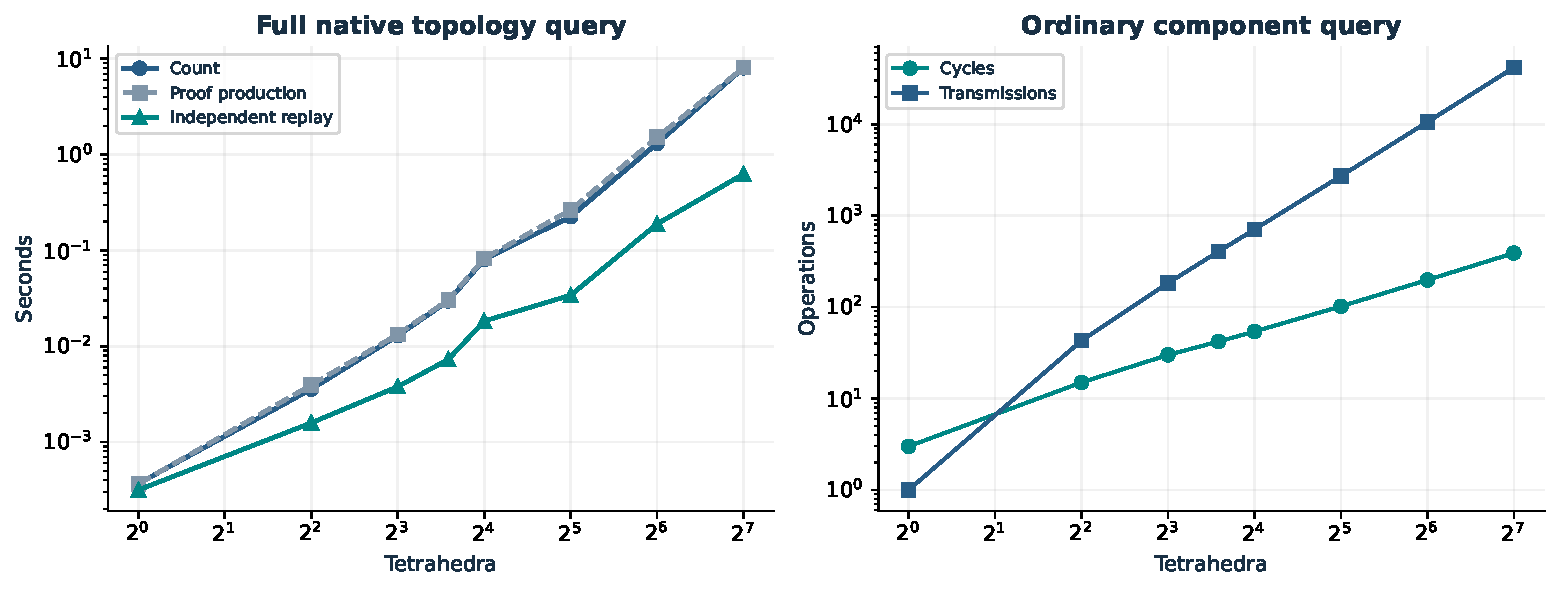
\includegraphics[width=\textwidth]{figures/normal_scaling.pdf}
\caption{Measured native topology costs and ordinary orbit work on supplied Fibonacci
meridian vectors. Lines join measured points only. They are not a fitted universal
complexity law.}\end{figure}

The small explicit controls are often faster. At $t=12$, literal polygon assembly
takes 9.659 ms versus 29.744 ms for the new aggregate query; Regina's component
routine takes 0.906 ms. At $t=16$, the literal control takes 98.205 ms versus
80.155 ms, while Regina remains faster at 3.226 ms. Those controls return a
different output protocol, and these figures are not claimed as certificate-level speedups.
Both explicit controls are restricted to at most 20,000 discs in the final benchmark.
Regina's documented \code{components()} routine explicitly constructs normal discs
\cite{reginadoc}; an initial uncapped diagnostic reached the 64-tetrahedron case
and raised \code{MemoryError: std::bad\_alloc}. Its aborted log is retained separately
and contributes no primary timing ratio. We then applied the same finite-oracle
cap to both explicit controls and reran the complete source-guarded benchmark.
The large rows therefore establish native compressed completion and proof replay,
not a fabricated ratio against a censored explicit computation.
